\documentclass[10pt]{beamer}
\usepackage[T1]{fontenc}
\usepackage[utf8]{inputenc}
\usepackage[french]{babel}
\usepackage{color}
\usepackage[normalem]{ulem}
\usepackage{soul}
\usetheme{Darmstadt}

\title{Le projet SAVOIE}
\subtitle{Formation à destination du superviseur - V0}
\author{Clovis HAMEL, Loïc PERRIN, Mickaël AMAND}
\date{T4 2018}

\AtBeginSection[]
{
  \begin{frame}<beamer>{Plan}
    \tableofcontents[currentsection,currentsubsection]
  \end{frame}
}
\AtBeginSubsection[]
{
  \begin{frame}<beamer>{Plan}
    \tableofcontents[currentsection,currentsubsection]
  \end{frame}
}

% Let's get started
\begin{document}

\begin{frame}
  \titlepage
\end{frame}

\begin{frame}{}
  \tableofcontents
  % You might wish to add the option [pausesections]
\end{frame}

\section{Introduction}
%%%%%%%%%%%%%%%%%%%%%%%%%%%%%%%%%%%%%%%%%%%
\section{Introduction}
%%%%%%%%%%%%%%%%%%%%%%%%%%%%%%%%%%%%%%%%%%%

\begin{frame}{Une prise de conscience nécessaire 1/2}
\begin{block}{Évolution des architectures applicatives}
\begin{itemize}
\item Applications client-serveur légers \pause
\item Recours aux technologies Web 2.0 (PHP, Javascript, Bootstrap, etc) \pause
\item Recours aux API (B2B Network Manager par exemple) \pause
\item Utilisation de technologies de conteneurisation telles que Docker \pause
\end{itemize}
\end{block}
\begin{block}{Évolution des méthodes de développement}
\begin{itemize}
\item Mise en retrait de la DTI \pause
\item Cycle de développement et de déploiement plus courts (cf ASAP, itérativité, etc) \pause
\item Diminution des RH mais contraintes maintenues \pause
\end{itemize}
\end{block}
\end{frame}

\begin{frame}{Une prise de conscience nécessaire 2/2}
\begin{block}{Evolution des méthodes de gestion de projet}
\begin{itemize}
\item Eviter l'effet tunnel en livrant plus souvent \pause
\item Déployer en continu \pause
\item Automatiser les tests (cf gitlab) \pause
\item Conserver une disponibilité maximum (sur panne et sur déploiement) par un retour arrière natif \pause
\end{itemize}
\end{block}
\end{frame}

\begin{frame}{Une dette technologique à combler}
\begin{block}{Un contrôle aérien qui a soif de modernité}
\begin{itemize}
    \item Décloisonnement des acteurs du TA (PC, FMP, CDS, Cie, NM, etc) \pause
    \item Numérisation et automatisation de l'information (\sout{téléphone})
    \item Une vitrine pour valoriser les compétences internes de la DSNA 
\end{itemize}
\end{block} 
 \begin{exampleblock}{Exemples d'applicatifs}
 WikiFF, 4Me, SALTO (sur SAVOIE), iStream, CCS (sur leur propre machines)
\end{exampleblock}
\begin{block}{Un existant peu optimal}
\begin{itemize}
\item Un bi-serveur par application (SIAM, EPEIRES, WikiFF)
\item Une box Internet par applicatif (iSTREAM, SALTO, etc)
\item Aucune mutualisation des services (3 applications sur SIAM-TECH, 3 serveurs MySQL)
\item Chaque section doit se former sur des méthodes de travail similaires 
\end{itemize}
\end{block}
\end{frame}

%%%%%%%%%%%%%%%%%%%%%%%%%%%%%
% Les solutions
%%%%%%%%%%%%%%%%%%%%%%%%%%%%%
\begin{frame}{Une solution en deux temps}
\begin{block}{Deux salles, deux ambiances, un même plaisir}
\begin{itemize}
    \item Une solution nationale : Le réseau ATM2 
    \item Une solution locale : L'infrastructure SAVOIE
\end{itemize}
\end{block} 

\begin{alertblock}{Nécessité de différencier les deux}
\begin{itemize}
    \item Pas les mêmes matériels
    \item Pas les mêmes intervenants nationaux et locaux impliqués
\end{itemize}
\end{alertblock} 

\begin{alertblock}{Mais les deux ne sont pas bijectifs ! \#ClassePrepa}
\begin{itemize}
    \item SAVOIE nécessite forcément ATM2 a priori ... \footnote{vSphere ne sert pas à virtualiser des clients. On peut le faire si on veut mais ce n'est pas fait pour. Au premier ordre, si on utilise SAVOIE pour implémenter un système, on utilisera ATM2. Si on ne veut pas utiliser ATM2, on utilise une infra indépendante.}
    \item Mais on peut connecter des systèmes sur ATM2 sans utiliser l'infrastructure SAVOIE. 
\end{itemize}
\end{alertblock} 
\end{frame}

\section{SAVOIE}
\subsection{Présentation et architecture}

\begin{frame}{SAVOIE bien ou quoi ?}
\begin{block}{Equipe projet}
\begin{itemize}
\item Chef de projet : S. HEURTIER + G. GUERIZEC 
\item Ensemble d'agents issus de toutes les subdivisions
\end{itemize}
\end{block}
\begin{block}{SAVOIE}
\begin{itemize}
\item Solution d’Architecture Virtuelle pour l’Opérationnel, Innovante et Évolutive  
\item Solution all-in-one d'hébergement à la sauce OVH, AWS  
\item Toponymie orientée autour du domaine skiable 3 vallées  
\end{itemize}
\end{block}
\begin{block}{Forces de l'infrastructure}
\begin{itemize}
\item Cluster de machines (en mode cattle, escadrille etc) \pause
\item Virtualisation des applicatifs \pause
\item Stockage partagé sur SAN  
\end{itemize}
\end{block}
\end{frame}

\begin{center}
\begin{frame}{Schéma d'infrastructure SAVOIE (WIP)}
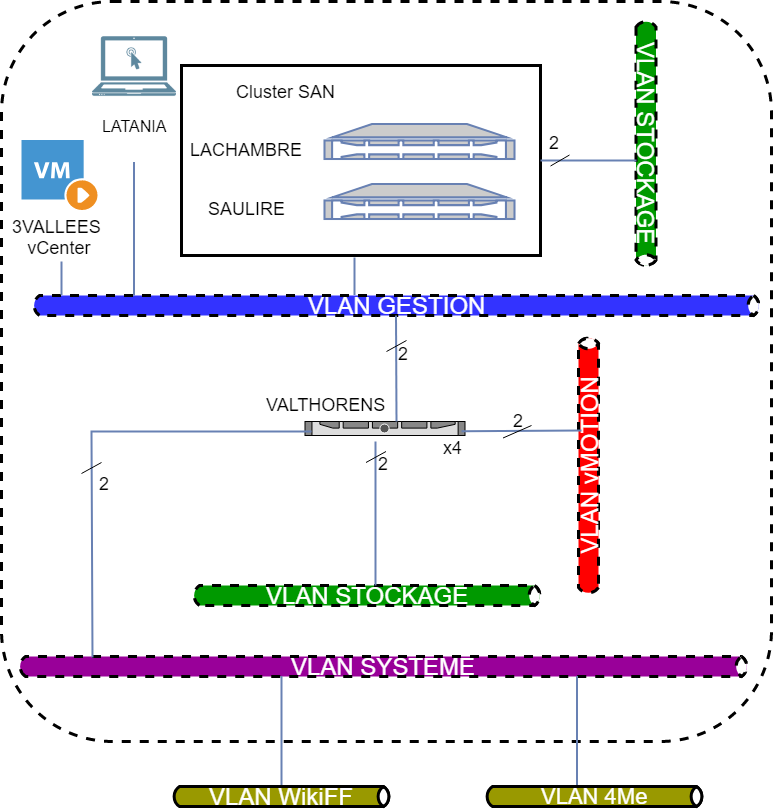
\includegraphics[width=200px]{Schemas/SAVOIE.png}
\end{frame}
\end{center}

\begin{frame}{Composition matérielle de la plate-forme}
\begin{block}{Sur le segment OPS}
\begin{itemize}
\item 4 ESX : lesmenuires.ops, valthorens.ops, meribel.ops et courchevel.ops
\item 2 SAN : lachambre.ops et saulire.ops
\item 1 station d'administration : latania.ops
\end{itemize}
\end{block}\pause
\begin{block}{Sur le segment PREOPS}
\begin{itemize}
\item 3 ESX : valthorens.preops, meribel.preops et courchevel.preops
\item 2 SAN : lachambre.preops et saulire.preops
\item 1 station d'administration : latania.preops
\end{itemize}
\end{block}
\end{frame}

\begin{frame}{Matériels SAVOIE}
\begin{block}{Quatre ESX}
\begin{itemize}
\item DELL R440 Intel Xeon E5 2.4GHz
\item 32GB de RAM 
\item 2 disques durs de 600GB en RAID 1 (miroir)
\item 4x1 GB Ethernet et une carte 4 ports 1 GB additionnelle
\end{itemize}
\end{block}
\begin{block}{Deux SAN}
\begin{itemize}
\item Synology RS818RP+
\item 4 disques durs Seagate Barracuda 6 To
\item Alimentation redondée
\item 4x1 GB Ethernet
\end{itemize}
\end{block}
\end{frame}


\begin{center}
\begin{frame}{Maquettage de la baie SAVOIE}
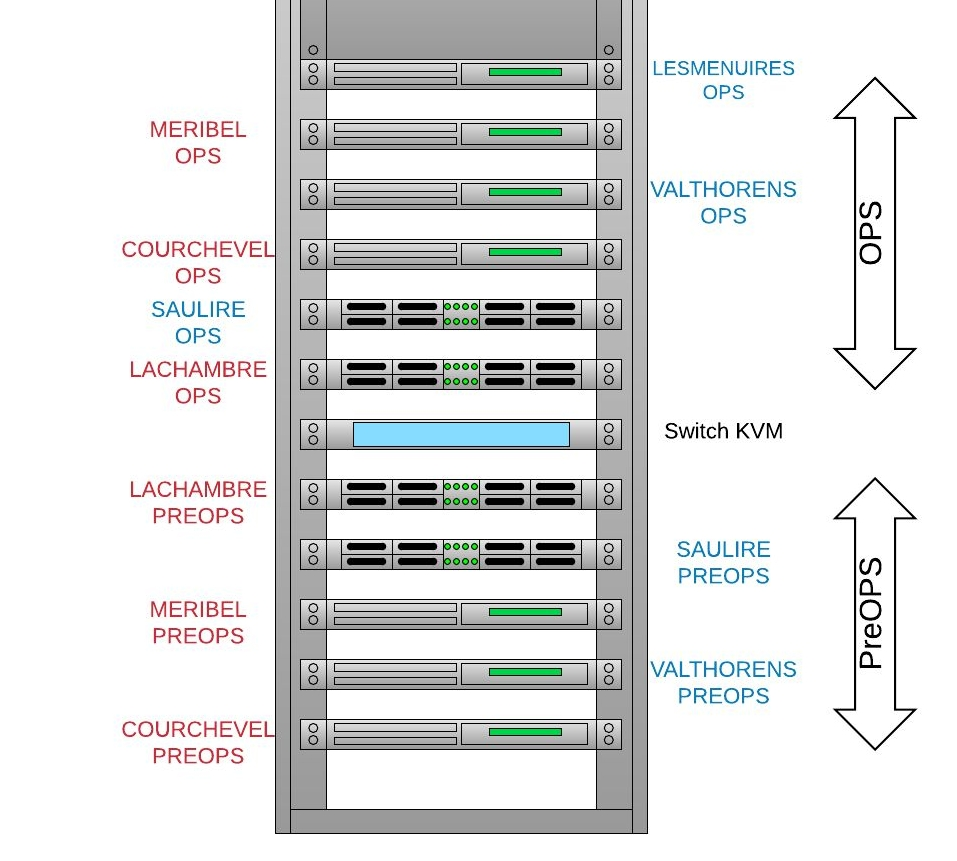
\includegraphics[width=250px]{Schemas/Maquettage_Savoie.jpg}
\end{frame}
\end{center}

\subsection{La virtualisation}

\begin{center}
\begin{frame}{La virtualisation}
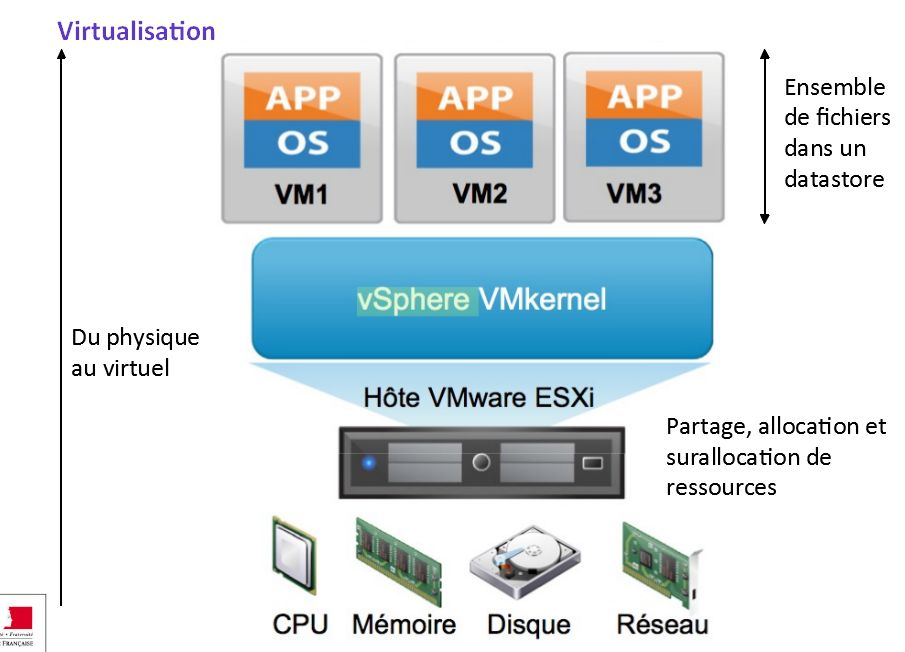
\includegraphics[width=300px]{Schemas/Virtua.jpg}
\end{frame}
\end{center}

\begin{frame}{Pourquoi virtualiser ? 1/2}
    \begin{block} {Rationalisation des équipements}
        \begin{itemize}
            \item Ratio machines/applications augmente => gain de performances, gain financier, gain écologique \pause
            \item Coimplantation de plusieurs applications avec des socles non compatibles (ou plusieurs versions d’un même applicatif) Ex : OASIS/ORFEO \pause
            \item Meilleure allocation des ressources en fonction des applicatifs (politique d'allocation plus fine, dynamique, sélective, etc) \pause
            \item Facilité de déploiement dans le cadre du devops \pause
            \item Backup, restore, snapshots facilités puisque une VM = des fichiers \pause
        \end{itemize}
    \end{block}
\end{frame}
        
    \begin{frame}{Pourquoi virtualiser ? 2/2}
        \begin{block} {Harmonisation et mutualisation des services}
        \begin{itemize}
        \item Les applicatifs s’abonnent aux services offerts dans le catalogue (base de données, apache, service de notifications, serveurs de log, serveur de dashboard/monitoring) \pause
        \item Déclinaison locale de la solution nationale ATMOS
        \end{itemize}
    \end{block}
    \end{frame}
        
\begin{frame}{Choix de l'hyperviseur VMware}
\begin{block}{Avantages}
\begin{itemize}
\item Leader du marché, gage de pérennité et de solidité \pause
\item Facilité pour trouver un prestataire de formation \pause
\item Solution complète au-delà de vSphere et vCenter (vCloud, vRealize, API SVG, etc) \pause
\item Régularité et réactivité au niveau des patchs et solutions de sécurité \pause
\item Interfaces graphiques conviviales et puissantes (Clickodrome) \pause
\item Expérience de Clément au travers de sa QTS et des ESX-TLC \pause
\end{itemize}
\end{block}
\begin{block}{Inconvénients}
\begin{itemize}
\item Coût financier important à rentabiliser \pause
\begin{itemize}
    \item Dès lors que le nombre d’applications hébergées est important \pause
\item Dès lors que le choix des licences est judicieux \pause
\end{itemize}
\item Coût RH important rentabilisé dès lors qu’on arrête d’installer N services identiques pour N projets 
\end{itemize}
\end{block}
\end{frame}

\begin{frame}{Intelligence névralgique : vCenter}
\begin{block}{La VM vCenter}
\begin{itemize}
\item Interface Web permettant de gérer un inventaire d’objets VMware de manière homogène et conviviale
\item Le vCenter est lui-même une VM que l’on déploie sur un ESX. On peut donc lui appliquer les mécanismes de HA de VMWare (vMotion, HA, FT)
\item Le vCenter permet de déployer de manière optimale les patchs de sécurité sur chaque ESX et sur vCenter lui-même
\item Nécessité de sauvegarder la configuration d’un vCenter de plus en plus critique
\end{itemize}
\end{block}
\end{frame}

\begin{frame}{Qu'est ce qu'une VM ?}
\begin{block}{Une VM est un ensemble de fichiers}
\begin{itemize}
\item \textbf{.VMDK} : Disque dur virtuel VMware. \pause
\item \textbf{.VMX }: Fichier de configuration de la machine virtuelle. Contient toutes les informations que vous paramétrez via l’interface graphique du logiciel. Exemples : nom de la machine, type d’OS, RAM, carte réseau, type de connexion,… \pause
\item \textbf{.VWSP} : Fichier d’échange (correspond au SWAP). \pause
\item \textbf{.VMSS} : Fichier qui enregistre l’état de la VM lorsqu’elle est suspendue (ce qui permet la reprise par la suite). \pause
\item \textbf{.NVRAM} : Fichier correspondant au BIOS de la VM   \pause
\item \textbf{.VMSN} : Contient l'état de la machine quand vous faite un snapshot (en créant un fichier par snapshot). \pause
\item \textbf{.LOG} : Enregistre les logs sur ce qu'il se passe sur la VM. 
\end{itemize}
\end{block} 
\end{frame}

%\begin{frame}{Schéma plus exhaustif}
%\begin{center}
%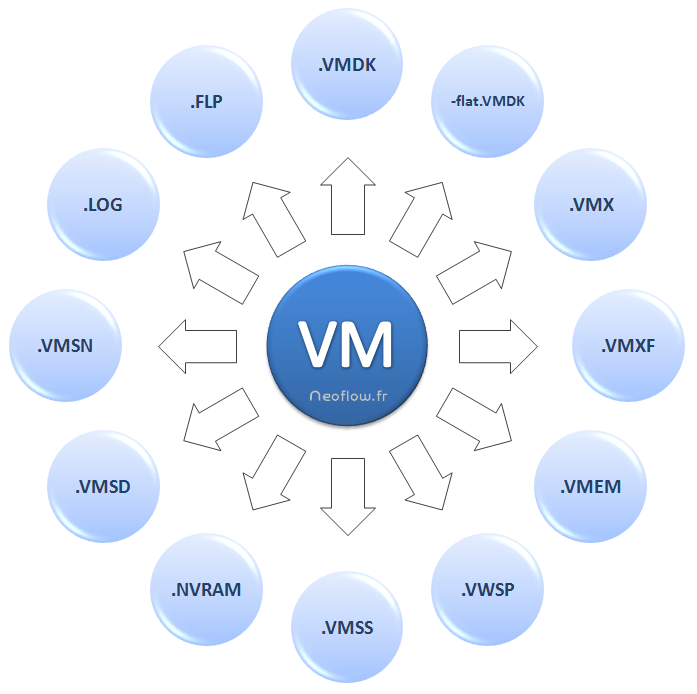
\includegraphics[width=230px]{Schemas/filevm.png}   
%\end{center}
%\end{frame}

\subsection{Stockage}
\begin{frame}{Le stockage dans SAVOIE}
\begin{block}{Principes}
\begin{itemize}
    \item Le stockage de SAVOIE repose sur deux SAN
    \item Clusterisation des SAN en mode maître-esclave
    \item Vu de l'extérieur, c'est comme si on n'avait qu'un seul SAN maître portant la @vIP
\end{itemize}
\end{block}
\end{frame}

\begin{frame}{Avantages et inconvénients d'un SAN}
\begin{block}{Avantages}
\begin{itemize}
    \item Avantage d'un stockage distant sur un stockage local
    \item Meilleure évolutivité
    \item Faire reposer une partie de la charge CPU sur les SAN \pause
\end{itemize}
\end{block}
\begin{block}{Inconvénients}
\begin{itemize}
          \item Forte dépendance au SAN
          \item Forte dépendance au réseau reliant le SAN aux ESX (VLAN STOCKAGE) en termes de performances et de disponibilité
\end{itemize}
\end{block}
\end{frame}

\begin{frame}{RAID 10}
\begin{block}{Fonctionnement}
\begin{itemize}
\item 2 disques en RAID0 : répartir les informations stockées sur plusieurs disques durs grâce à un entrelacement des données. Temps d'accès accéléré.
\item 2 disques en RAID1 : l’un est utilisé en miroir de l'autre
\end{itemize}
\end{block}
\begin{block}{Avantages et inconvénients}
\begin{itemize}
\item Permet la performance et la disponibilité
\item Performance de 50\% (4*6To=>12To)
\end{itemize}
\end{block}
\end{frame}

\begin{frame}{Comment le stockage est-il réalisé dans SAVOIE ?}
\begin{center}
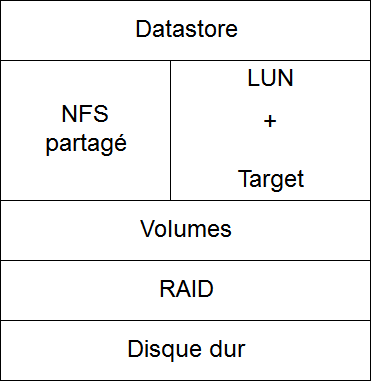
\includegraphics[width=200px]{Schemas/Concepts_Stockage.png}
\end{center}
\end{frame}


\subsection{Réseaux virtuels}
\begin{frame}{Deux fonctionnalités réseaux utilisées dans SAVOIE : Isolation des flux}
\begin{block}{Quatre VLAN tagués sont utilisés}
\begin{itemize}
\item GESTION pour administrer les ESX et les SAN via un poste d'administration (LATANIA) \pause
\item vMOTION pour la migration des VM d'un ESX à un autre \pause
\item STOCKAGE pour les lectures et écritures sur le SAN \pause
\item SYSTEME sur lequel les VM applicatives serveurs communiquent avec les clients physiques \pause
\end{itemize}
\end{block}
\begin{block}{Pourquoi isoler les flux ?}
\begin{itemize}
    \item Préconisation de l'ANSSI \pause
    \item Allocation de ressources indépendantes et dédiées (Ex : Un VLAN GESTION a besoin de moins de ressources qu'un VLAN STOCKAGE)
\end{itemize}
\end{block}
 
\end{frame}

\begin{frame}{Deux fonctionnalités réseaux utilisées dans SAVOIE : Agrégation de liens réseaux}
\begin{block}{Avantages}
\begin{itemize}
\item Augmente la disponibilité réseaux en cas de perte d'un lien
\item Augmente le débit disponible pour une artère
\end{itemize}
\end{block}
\begin{block}{Inconvénients}
\begin{itemize}
\item Besoin d'un grand nombre de cartes Ethernet sur un ESX (8 dans SAVOIE, maximum possible simplement chez DELL)
\end{itemize}
\end{block} 
\begin{block}{Dans SAVOIE}
\begin{itemize}
\item Agrégation de 2 cartes pour GESTION, vMOTION, STOCKAGE et SYSTEME
\item Augmente le débit disponible pour une artère
\end{itemize}
\end{block}
\end{frame}

\begin{frame}{La Base}
    \begin{center}
    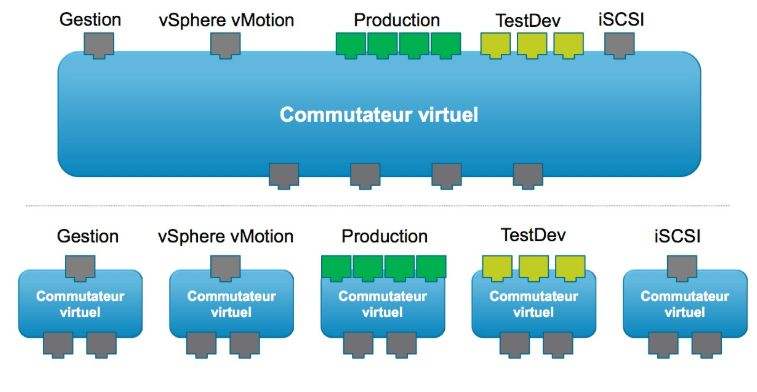
\includegraphics[width=300px]{Schemas/Commu.jpg}
    \end{center}
\end{frame}

\begin{frame}{Vu de l'ESX}
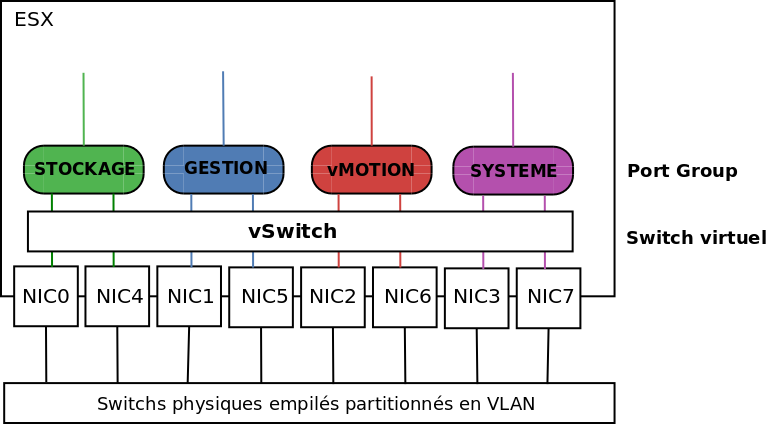
\includegraphics[width=300px]{Schemas/VLAN.png}
\end{frame}

\begin{frame}{Vu du SAN}
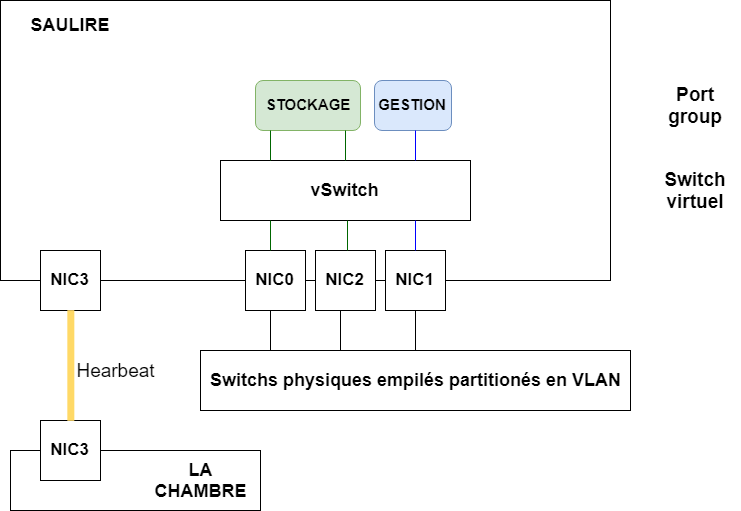
\includegraphics[width=300px]{Schemas/VuDuSan.png}
\end{frame}


\subsection{Les fonctionnalités VMware}
\subsection{Les fonctionnalités VMware}

\begin{center}
\begin{frame}{vMotion}
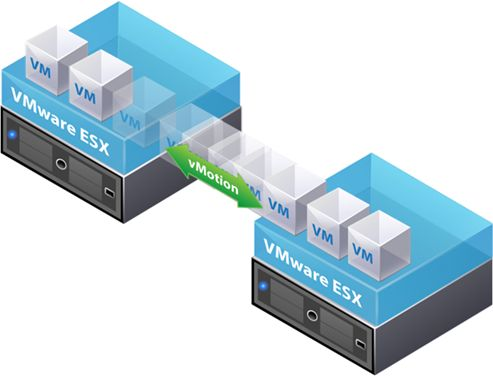
\includegraphics[width=260px]{Schemas/vMotion.jpg}
\end{frame}
\end{center}

\begin{center}
\begin{frame}{Storage vMotion}
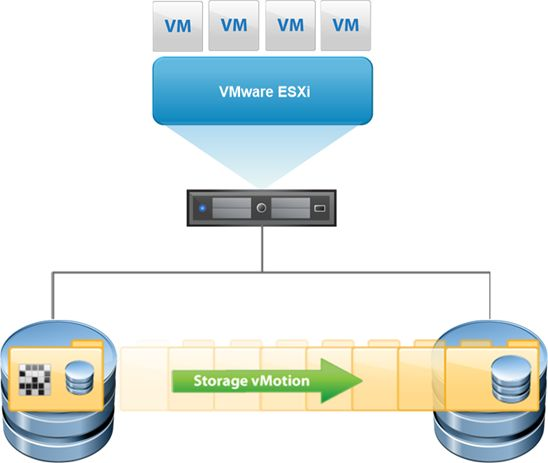
\includegraphics[width=250px]{Schemas/Storage_vMotion.jpg}
\end{frame}
\end{center}

\begin{center}
\begin{frame}{Thin Provisionning vs Thick Provisionning}
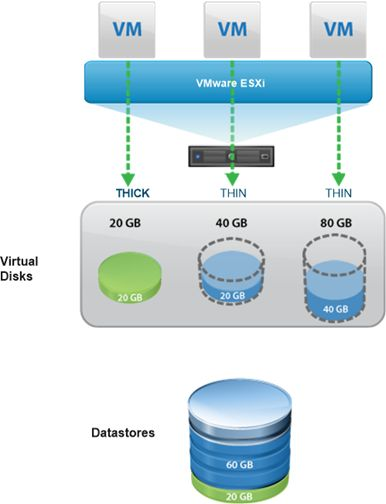
\includegraphics[width=150px]{Schemas/Thin_Provisionning.jpg}
\end{frame}
\end{center}

\begin{center}
\begin{frame}{High Availability (HA)}
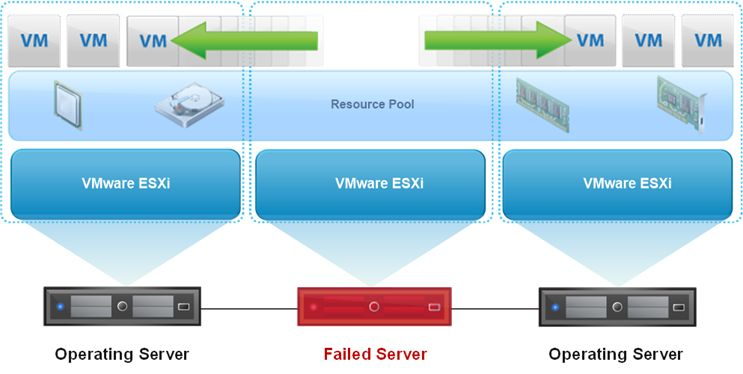
\includegraphics[width=310px]{Schemas/High_Aviability.jpg}
\end{frame}
\end{center}

\begin{center}
\begin{frame}{Fault Tolerance (FT)}
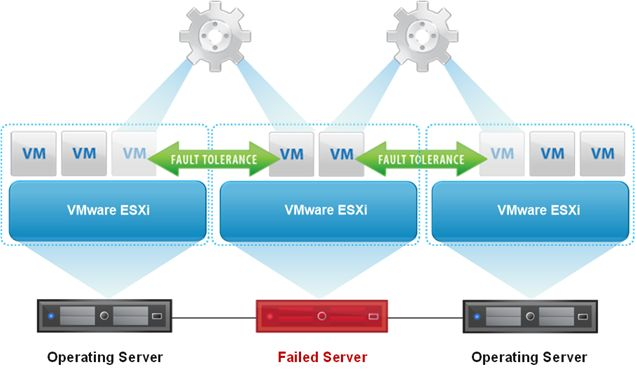
\includegraphics[width=310px]{Schemas/Fault_Tolerance.jpg}
\end{frame}
\end{center}

\section{Maintenance Opérationnelle}
\begin{frame}{MESO}
\begin{block}{Une MESO progressive}
\begin{itemize}
\item 1er Octobre : MESO SAVOIE (sans applicatifs)
\item 1er Novembre : MESO WikiFF sur positions et CDS via ATM2/SAVOIE
\end{itemize}
\end{block}
\begin{block}{Une MO répartie sur deux superviseurs}
\begin{itemize}
\item Les superviseurs RVU (resp CAW) utilisent leur casquette ODA (resp CAU) pour superviser SAVOIE
\item Les superviseurs RVU (resp CAW) utilisent leur casquette ODR (resp WAN) pour superviser ATM2
\item Pour chaque applicatif tournant dans la VM, le superviseur reste inchangé. Ex : WikiFF (RVU), 4Me (CAW)
\item Pour le début, il n'y aura qu'un SPV de formé \textit{a minima}. 
\end{itemize}
\end{block}
\end{frame}

\begin{frame}{Que doit faire le superviseur ?}
\begin{block}{Processus en trois temps}
\begin{itemize}
\item Identifier
\item Communiquer
\item Agir
\end{itemize}\pause
\end{block}
\begin{block}{Outils à la disposition des superviseurs}
\begin{itemize}
\item La station d'administration LATANIA
\item Le supervision applicative (WIP)
\item SIAM (WIP)
\end{itemize}
\end{block}
\end{frame}

\begin{frame}{Identifier et Communiquer}
\begin{block}{Identifier l'incident}
\begin{itemize}
\item Identifier une panne de composants (ESX, SAN, disque, etc)
\item Identifier la "bonne santé" d'une VM (i.e savoir si le problème vient de SAVOIE ou de l'application)
\end{itemize}\pause
\end{block}
\begin{block}{Communiquer}
\begin{itemize}
\item Aux utilisateurs l'impact et le temps de rétablissement
\item à la MS les infos les plus pertinentes possibles pour aider à la résolution du problème
\end{itemize}
\end{block}
\end{frame}

\begin{frame}{Agir}
\begin{block}{Agir sur une VM}
\begin{itemize}
\item Arrêter/Démarrer une VM dégradée ou en panne
\end{itemize}
\end{block}
\begin{block}{Agir sur les ESX}
\begin{itemize}
\item \textcolor{red}{Aucun changement d'ESX n'est fait par la MO}
\end{itemize}
\end{block}
\begin{block}{Agir sur les SAN}
\begin{itemize}
\item \textcolor{red}{Aucun changement de disque SAN n'est fait par la MO}
\item \textcolor{red}{Aucun changement de SAN n'est fait par la MO}
\end{itemize}
\end{block}
\end{frame}

\section{Partie pratique}
\begin{frame}{Repérer les différents équipements dans la baie SAVOIE}
\begin{block}{En salle technique}
    \begin{itemize}
        \item Segment OPS et PREOPS
        \item Les ESX
        \item Les SAN
    \end{itemize}
\end{block}
\end{frame}

\begin{frame}{Interfaces Web à disposition}
    \begin{itemize}
        \item Interface relative à un ESX
        \item Interface relative au vCenter
        \item Interface relative au SAN 
    \end{itemize}
\end{frame}

\begin{frame}{Adressage réseaux de la plateforme}
A l'aide des interfaces Web, remplir les tableaux suivants avec les adresses IP virtuelles des ESX.
\\
\begin{center}
 \begin{tabular}{|c || c | c | c | c|} 
 \hline
  & GESTION & vMOTION & STOCKAGE & SYSTEME \\ [0.5ex] 
 \hline
 valthorens &  &  & & \\ [0.5ex]
 \hline
 courchevel &  &  & &  \\ [0.5ex]
 \hline
 meribel &  &  &  &  \\ [0.5ex]
 \hline
 saulire &  &  &  &  \\ [0.5ex]
 \hline
 lachambre &  &  &  &  \\ [0.5ex]
 \hline
 latania  &  &  &  &  \\ [0.5ex]
 \hline
\end{tabular}
\end{center}
\end{frame}

\begin{frame}{Exercice}
\begin{block}{Enoncé}
\begin{itemize}
\item Création d'une VM \textit{\textbf{magasinier}} utilisant le datastore distant \textbf{\textit{entrepot}}
\end{itemize}
\end{block}
\begin{block}{Caractéristique de la VM magasinier}
\begin{itemize}
\item 2 GB de RAM
\item Utilise un OS Linux
\item Est connecté au moins à un réseau \textbf{\textit{ligne2prod}}
\end{itemize}
\end{block}
\begin{block}{Caractéristique du datastore entrepot}
\begin{itemize}
\item 25 Go Thin provisioning
\item Systeme de fichiers VMFS
\end{itemize}
\end{block}
\end{frame}

\begin{frame}{Jouons un peu avec notre VM}
\begin{block}{Etat de santé de la VM}
\begin{itemize}
\item Graphiques montrant la charge CPU et l'utilisation de la RAM
\end{itemize}
\end{block}
\begin{block}{Test du vMotion}
\begin{itemize}
\item Migrer la VM magasinier sur un autre ESX. 
\item Regarder le temps de traitement, la charge réseau sur les ESX, les logs.
\end{itemize}
\end{block}
\end{frame}

\begin{frame}{VM et datastore}
\begin{block}{Une VM, c'est quoi déjà ?}
\begin{itemize}
\item Où peut-on trouver concrètement la VM magasinier sur le SAN ? 
\item Renommer le fichier vm-magasinier.VMDK en vm-marsouin.VMDK. Que se passe-t-il ? Pourquoi ? 
\item Renommer le fichier correctement
\end{itemize}
\end{block}
\end{frame}

\begin{frame}{Exercice}
\begin{block}{Enoncé}
\begin{itemize}
\item Dans la VM, créer sur le bureau un fichier texte nommé "Marseille" et y inscrire dedans une phrase quelconque.
\item Voyons comment faire un snapshot de la VM (expliquer ce qu'est un snapshot rapidement)
\item Regardons dans le datastore entrepôt le fichier créé
\item Simuler une erreur d'un agent en détruisant le fichier Marseille.
\item Utiliser la gestion des snapshots pour revenir à l'état initial de la VM et ainsi s'apercevoir que l'erreur a été corrigée.
\end{itemize}
\end{block}
\begin{alertblock}{Attention}
\begin{itemize}
\item L'utilisation des snapshots n'est pas une méthode de sauvegarde de VM
\end{itemize}
\end{alertblock}
\end{frame}

\begin{frame}{Cas de pannes : ESX}
\begin{block}{ESX}
\begin{itemize}
\item Eteindre proprement l'ESX sur lequel tourne la VM magasinier. Que se passe-t-il ?
\item Regardons les logs
\item Redémarrer proprement l'ESX et attendre la remise en conformité de la plate-forme
\end{itemize}
\end{block}

\begin{block}{Cas de pannes : ESX ft vMotion}
\begin{itemize}
\item Créer un cluster et y inclure la VM Magasinier
\item Eteindre proprement l'ESX sur lequel tourne la VM magasinier. Que se passe-t-il ?
\item Regardons les logs
\item Redémarrer proprement l'ESX et attendre la remise en conformité de la plate-forme
\end{itemize}
\end{block}
\end{frame}

\begin{frame}{Cas de pannes 2}
\begin{block}{Cas de pannes : SAN}
\begin{itemize}
\item Eteindre proprement le SAN maître. Que se passe-t-il dans la VM ?
\item Si on ne dispose que d'un SAN sur la plateforme, éteindre proprement le SAN. Que se passe-t-il ?
\item Regardons les logs
\item Redémarrer proprement le SAN et attendre la remise en conformité de la plate-forme
\end{itemize}
\end{block}
\end{frame}

\begin{frame}{Cas de pannes 3}
\begin{block}{Cas de pannes : Réseaux}
\begin{itemize}
\item Repérer une NIC relative au VLAN STOCKAGE. La déconnecter du switch.
\item Que se passe-t-il au niveau de la VM ?
\end{itemize}
\end{block}

\begin{block}{Cas de pannes : Réseaux}
\begin{itemize}
\item Réperer une NIC relative au VLAN vMotion. La déconnecter du switch.
\item Que se passe-t-il au niveau de la VM ? 
\item Eteindre l'ESX hébergeant la VM magasinier. Que devrait-il se passer ? Que se passe-t-il ? Pourquoi ?
\end{itemize}
\end{block}
\end{frame}

\begin{frame}{Avant de partir ...}
\begin{block}{Remise en conformité de la plateforme}
\begin{itemize}
\item Supprimer la VM magasinier du datastore
\item Supprimer le cluster
\item Supprimer les réseaux créés
\item Supprimer toutes les modifications que l'on a apportées sur les SAN
\item Vérifier que les ESX et les SAN sont allumés
\item Vérifier les branchements réseaux
\end{itemize}
\end{block}
\end{frame}

\end{document}